In the earlier sections the preliminaries and model frame were introduced and expained. In this section the model validation and results of simulating will be analysed in Section \ref{sec:valid_no_ILC} without the higher-layer control and in Section \ref{sec:valid_ILC} with. The discussion of the results will take place in Section .
\\The code of the nonlinear model is written in Julia 1.4.0 and
is available on request or on github. The simulations were performed using the DifferentialEquations.jl package, Rackauckas and Nie (2017), and the Rodas4p solver, Wanner and Hairer (1996).
\\For the model validation and the result representation we consider a fully connected microgrid of 4 nodes ($N=4$, see notations at Section \ref{subsec:prosumermodel}). Every node has a local low-level controller as well as a high-level controller, i.e., without additional communication \cite{paperilc}. The model parameters are summarized in Table \ref{tab:parameters}.

% Please add the following required packages to your document preamble:
% \usepackage{booktabs}
% \usepackage{multirow}
\begin{table}[htbp]
	\centering
	\footnotesize
	\begin{tabular}{@{}lllll@{}}
		\toprule
		\textbf{Level}              & \textbf{Symbol} & \textbf{Value}        & \textbf{SI Unit}  & \textbf{Description}                                        \\ \midrule
		\multirow{3}{*}{}           & $N$             & $4$                   & -                 & number of grid nodes in the network                         \\
		& $j$             & $1,2,3,4$             & -                 & grid nodes in the network                                   \\
		& $jk$            & $1,2,3,4,5,6$         & -                 & power lines in the network                                  \\ \midrule
		\multirow{5}{*}{low-level}  & $C_{cap,j}$     & 0.01                  & $\si{\farad}$          & given capacitance of the capacitor at the grid node         \\
		& $L_{pl,jk}$     & $0.237\cdot 10^{-4}$  & $\si{\henry}$          & given power line inductance                                 \\
		& $R_{pl,jk}$     & $0.532 \cdot 10^{-1}$ & $\si{\ohm}$            & given power line resistance                                 \\
		& $v_{gn,j}$      & $48$                  & $\si{\volt}$           & given reference voltage of the microgrid                    \\
		& $K_{D,j}$         & varies                  & $\frac{1}{\si{\ohm}}$  & droop coefficient of the prosumer                           \\ \midrule
		\multirow{2}{*}{high-level} & $\kappa$        & varies                  & $\frac{1}{\si{\hour}}$ & learning parameter                                          \\
		& $f_c$           & $\frac{1}{6}$         & -                 & relative cutoff frequency of Butterworth lowpass filter $Q$ \\ \bottomrule
	\end{tabular}
\caption{Values of parameters}
\label{tab:parameters}
\end{table}
\section{Model validation and results of the network without higher-layer control and periodic load profiles}
\label{sec:valid_no_ILC}
To model the direct current prosumer-based microgrid network it is analyzed the compound plant, i.e. only the network model with lower-layer control at first. Figures \ref{fig:current_no_ILC} and \ref{fig:voltage_no_ILC} are the simulated currents per edge/power line and voltages per node. The voltage reference per node amounts $V_{ref,j} = \SI{48}{\volt}$ and the node voltages oscillate in an interval $I = [\SI{47}{\volt},\SI{48}{\volt}]$, as seen in Figure \ref{fig:voltage_no_ILC}.
\subsubsection*{Interpretation}
 Assuming that the difference of node voltage and reference voltage should not exceed a value of $\SI{2}{\volt}$,so:
\begin{align*}
|v_{gn,j}(t)-V_{ref,j}| &\leq \SI{2}{\volt}, \forall t \in \mathbb{R}, j=1,2,3,4
\end{align*}
one can see that the control objective (\ref{enum:bounded_voltage}) of Section \ref{subsec:conobj} is respected. 
\\Control objective \ref{enum:power_sharing} states for the power sharing of the prosumers. When the time deriatives are zero, i.e. the highest and lowest values of the node powers, it can be seen in Figure \ref{fig:power_no_ILC} that every node feeds almost the same amount of power into the grid. The difference of the peaks of power for every node is max. $\SI{1}{\watt}$. Section \ref{sec:valid_ILC} refers to the validation of the network model with the iterative learning control.
\begin{figure}[h]
	\centering
	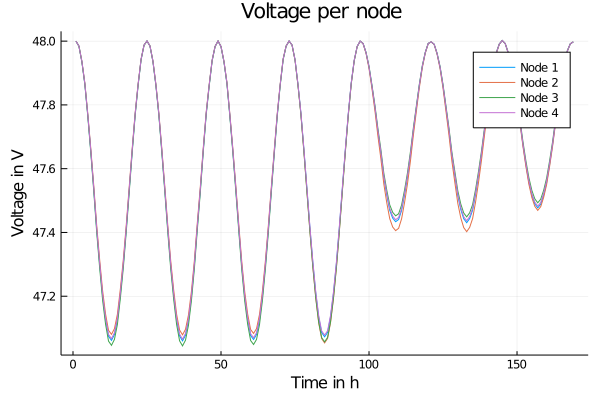
\includegraphics[scale=0.45]{pictures/plots/DC_prosumer_no_ILC_voltage_per_node.png}
	\caption{Voltage $v_{gn,j}(t)$ per node $j=1,2,3,4$ with no higher-layer control for 7 days in hours}
	\label{fig:voltage_no_ILC}
\end{figure}
\begin{figure}[h]
	\centering
	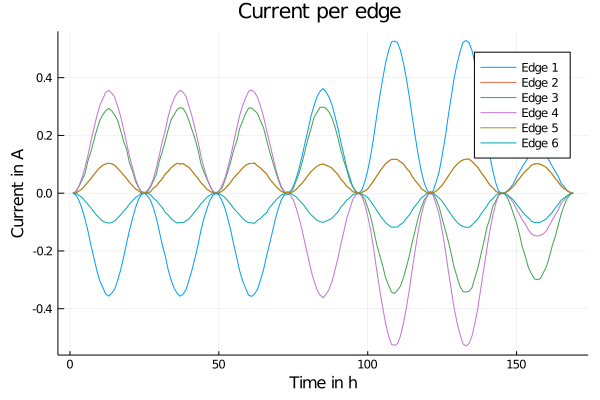
\includegraphics[scale=0.45]{pictures/plots/DC_prosumer_no_ILC_current_per_edge.png}
	\caption{Current per edge with no higher-layer control for 7 days in hours}
	\label{fig:current_no_ILC}
\end{figure}
\begin{figure}[h]
	\centering
	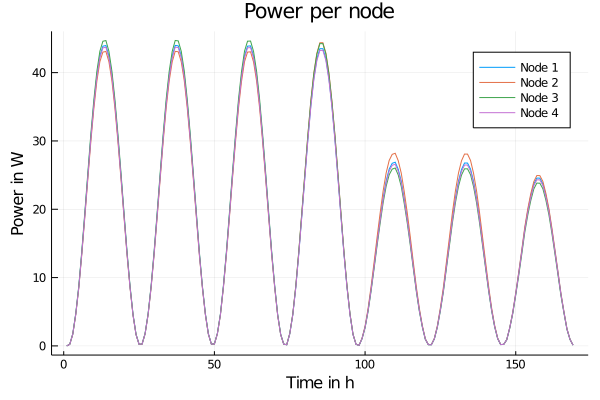
\includegraphics[scale=0.45]{pictures/plots/DC_prosumer_no_ILC_power_per_node.png}
	\caption{Low-level control energy with no higher-layer control for 7 days in hours}
	\label{fig:power_no_ILC}
\end{figure}
\section{Model validation and results of the network with higher-layer control and periodic load profiles}
\label{sec:valid_ILC}
For this section, we now consider the complete derived model of the prosumer-based direct current fully connected microgrid with the iterative learning control and without additional communication. The values of the parameters can be taken from Table \ref{tab:parameters}. 
\\In order to validate the proposed hierarchical controller and to discuss the behavior of it, the two control parameters, the learning parameter of the ILC $\kappa$ and the droop coefficient of the lower-layer control $\boldsymbol{K_D}$ will be varied, so that different case distinctions arise. In particular, we will observe the following cases:
\begin{itemize}
	\item \textbf{Case 1:} Validation of the network modeling with $K_{D,j} = 1$ and $\kappa = 1$ (\ref{subsec:case1})
	\item \textbf{Case 2:} Variation of $\boldsymbol{K_D}$, $\kappa = 1$ (\ref{subsec:case2})
	\item \textbf{Case 3:} Variation of $\kappa$, $K_{D,j} = 1$ (\ref{subsec:case3})
	\item \textbf{Error dynamics for different learning gains}
\end{itemize}
\subsection{Case 1: Validation of the network modeling with $\boldsymbol{K_{D,j} = 1}$ and $\boldsymbol{\kappa = 1}$}
\label{subsec:case1}
Case 1 serves the purpose to validate the overall nonlinear system model (\ref{eq:system}), (\ref{eq:ll_energy}) (\ref{eq:control_ilc}). The main results of case 1 are presented in the following.
\subsubsection*{Description}
Figure \ref{fig:energy_bilance} shows the injected power at the grid nodes. Recall that this is not the low-level control energy. Furthermore, it is the power that is calculated by the product of the voltages $v_{gn,t}(t)$ and the injected currents $i_{gn,t}(t)$ at the grid nodes. 
\\Figure \ref{fig:k1_K1} shows the sum over all nodes of the demand $P_j^d$ (transparent blue), the hourly integrated low-level control energy $y_j^{c,h}$ (red line) and the input from the ILC $u_j^{ILC}$ (black line) for a learning scenario with daily step changes of the peak demand. The peak demand is stepping after four days and again after three or four more days  and is different at each node (Figure \ref{fig:k1_K1}, bottom).As soon as the peak demand steps the low-layer control energy increases on the same day and decreases again on the next day. E.g. a peak of the energy of approx. $\SI{50}{\watt}$ appears on day 5. 

\subsubsection*{Interpretation}
Regarding the injected power of Figure \ref{fig:energy_bilance}, for every hour of the 7 days, the node energies are balanced and power sharing is achieved. This means that if at least one node produces an specific amount of energy, then the remaining node(s) consume this amount, the sum of all injected powers at every grid node is zero. 

Regarding the two-layer control (Figure \ref{fig:k1_K1}) it can be observed that the local ILC learns the local demand. It also steps after four days with a one-day delay (since on Day 1 the ILC does not have learned anything yet). By observing the low-level control energy it can also be determined, that power sharing in the network is achieved through the low-layer control input $u_j^{LI}$ from the first day. The sum of the lower-layer control energy $y^{c,h,s} = \sum_{j}y^{c,h}_j$ is distributed on all 4 nodes proportionally for every $K_{D,j} \in \mathbb{R}_{>0}$ (homogenous scenario).
The following relationship (for every amount of prosumer-nodes) arises:
\begin{align}
N \cdot K_{D,j} \cdot y^{c,h}_j &= y^{c,h,s}, N \in \mathcal{N} \subseteq \mathbb{N}, j={1,2,...,N}, K_{D,j} \in \mathbb{R}_{>0} \label{eq:sum_energy_hom} \\
4 \cdot y^{c,h}_j &= y^{c,h,s} ,N=4, K_{D,j}=1, j=1,2,3,4 \nonumber
\end{align}
Furthermore, the ILC learns based on the synchronized state for the whole network reducing successfully the lower-layer control energy at all nodes. The results of the summed quantities show that, after each demand peak step the ILC learns to compensate the new demand and thereby decreases the low-level control energy to less than $10\%$ of its original value within two days.
\\The fast increase of low-level control energy during the fifth day occurs, since the ILC has not learned yet the new peak demand and therefore reacts by not being able to keep the low-level energy small.
\\Case 1 serves as the "\textit{default}" case for the purpose of validating the network modeling. However, both the low-level and higher-layer controller must be tested in further cases to clarify the conclusions. E.g. in the next case the influence of the control parameter $K_{D,j}$ will be analyzed to confirm the proposed control objectives of power sharing and bounded voltage (\ref{subsec:conobj}).
\begin{figure}[h]
	\centering
	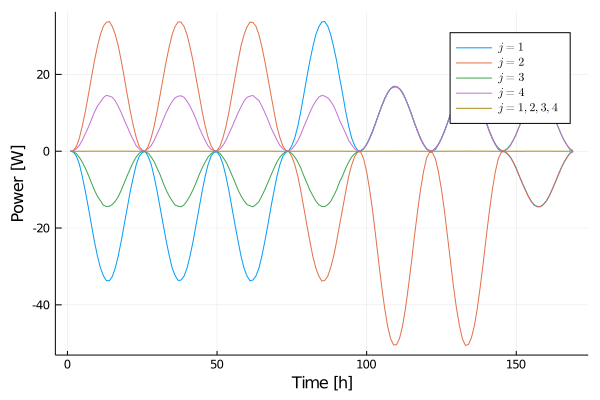
\includegraphics[scale=0.6]{pictures/plots/manual_calc_variation_kappa/kappa_1/K_1/energy_bilance.png}
	\caption{Injected power at every node $j=1,2,3,4$ and the sum (yellow line)}
	\label{fig:energy_bilance}
\end{figure}  
\begin{figure}[h]
	\centering
	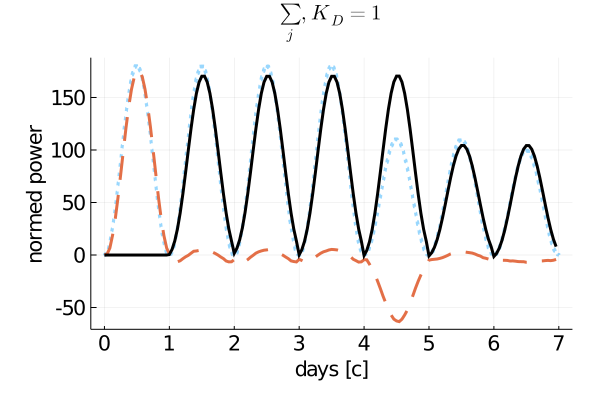
\includegraphics[scale=0.55]{pictures/plots/manual_calc_variation_kappa/kappa_1/K_1/DC_prosumer_demand_seconds_sum_hetero.png}
	
	\bigbreak
	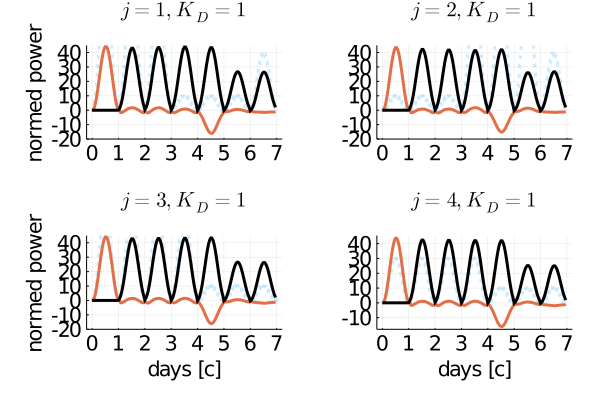
\includegraphics[scale=0.55]{pictures/plots/manual_calc_variation_kappa/kappa_1/K_1/DC_prosumer_demand_seconds_nodes_hetero.png}
	
	
	
	\caption{Top: sum for all nodes $j = 1,2,3,4$, $\kappa = \SI{1}{\hour ^{-1}}$ and $K_{D,j} = \SI{1}{\ohm ^{-1}}$; transparent blue: $\sum_{j} P_j^d$, dashed red: $\sum_{j} y_j^{c,h}$, solid black: $\sum_{j}u_j^{ILC}$; Bottom: seperately for nodes $j = 1,2,3,4$, $\kappa = \SI{1}{\hour ^{-1}}$, $K_{D,j} = \SI{1}{\ohm ^{-1}}$; transparent blue: $P_j^d$, solid red: $y_j^{c,h}$, solid black: $u_j^{ILC}$}
	\label{fig:k1_K1}
\end{figure}

\subsection{Case 2: Variation of  $\boldsymbol{K_D}$ and $\boldsymbol{\kappa = 1}$}
\label{subsec:case2}
Case 2 serves the purpose of analyzing the learning behavior of the hierarchical control for different droop coefficients $K_{D,j}, j=1,2,3,4$ and the influence of this coefficient on the power sharing. For this, K will be set to a vector of different values in order to examine how the variation of droop coefficients affects (quantitatively) the low-level energy. 
\subsubsection*{Description}
Note that the coefficient determines the voltage drop at the output, in our case the difference $V_{ref,j} - v_{gn,j}(t), j=1,2,3,4$.Two different \textit{heterogeneous} scenario have been selected for this case, where different droop coefficients are applied for every node. \textit{Homogeneous} scenarios include the same coefficients on every node. The following droop coefficients $\boldsymbol{K_D} = (K_{D,1},K_{D,2},K_{D,3},K_{D,4})^T$ were used:
\begin{align*}
\boldsymbol{K_{D,a}} = \left(\begin{array}{c} 0.1 \\ 1 \\2\\5 \end{array}\right)\si{\ohm^{-1}} , \boldsymbol{K_{D,b}} = \left(\begin{array}{c} 1 \\ 1 \\0.1\\1 \end{array}\right)\si{\ohm^{-1}} 
\end{align*}
Four different values have been assigned for every node in $\boldsymbol{K_{D,a}}$ and one different value in $\boldsymbol{K_{D,b}}$.
Figures \ref{fig:k1_KDa} and \ref{fig:k1_KDb} show the demand $P_j^d$ (transparent blue), the hourly integrated low-level control energy $y_j^{c,h}$ (red line) and the input from the ILC $u_j^{ILC}$ (black line) and the sums $\sum_{j}P_j^d$, $\sum_{j}y_j^{c,h}$ and $\sum_{j}u_j^{ILC}$ for learning scenarios with daily step changes of the peak demand for the droop coefficient $\boldsymbol{K_{D,a}}$ and $\boldsymbol{K_{D,b}}$, respectively, $j=1,2,3,4$. 

\paragraph{$\boldsymbol{K_{D,a}}$:} 
Changing the droop coefficient for every node obviously changes also the value of the daily low-level control energy. E.g. in node 1, the droop coefficient $K_{D,a,1} = \SI{0.1}{\ohm^{-1}}$ was applied. Since this parameter is also an immediate part of $u^{LI}$ (Eq. \ref{eq:ll_energy}) the hourly integrated energy is reduced by almost $\frac{1}{10}$ compared to the energy on node 2 with $K_{D,a,2} = \SI{1}{\ohm^{-1}}$ . However, the energy on node 2 is smaller than the energies in Case 1 ($K_{D,j} = \SI{1}{\hour^{-1}}$). For node 4, the droop coefficient $K_{D,a,4} = \SI{5}{\ohm^{-1}}$ was applied. The integrated energy in this node is almost 5 times bigger compared to node 2. Increased, i.e. decreased lower-layer control energy leads to equivalently increased, i.e. decreased ILC power, which can also be observed in Figure \ref{fig:k1_KDa}. The sum of powers on each node is observed to be equivalent compared to Case 1 ($K_{D,j} = \SI{1}{\hour^{-1}}$). 
\paragraph{$\boldsymbol{K_{D,b}}$:}
In this case, it is observed that that nodes $j=1$, $j=2$ and $j=4$, where the droop coefficient $\SI{1}{\hour^{-1}}$ is applied show the same amount of low-level control energy. The energies are bigger than the Case 1 ($K_{D,j} = \SI{1}{\hour^{-1}}$) energies with the same droop coefficient. For node $j=3$ with $K_{D,b,3} = \SI{0.1}{\hour^{-1}}$ the energy is reduced by almost $\frac{1}{10}$ compared to the other nodes. The sum of powers on each node is equivalent compared to Case 1 ($K_{D,j} = \SI{1}{\hour^{-1}}$). 
\begin{figure}[h]
	\centering
	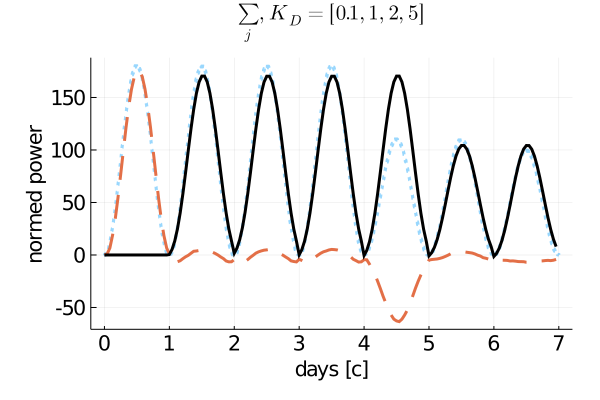
\includegraphics[scale=0.55]{pictures/plots/manual_calc_variation_kappa/kappa_1/K_variance/KDa/DC_prosumer_demand_seconds_sum_hetero.png}

	\bigbreak
	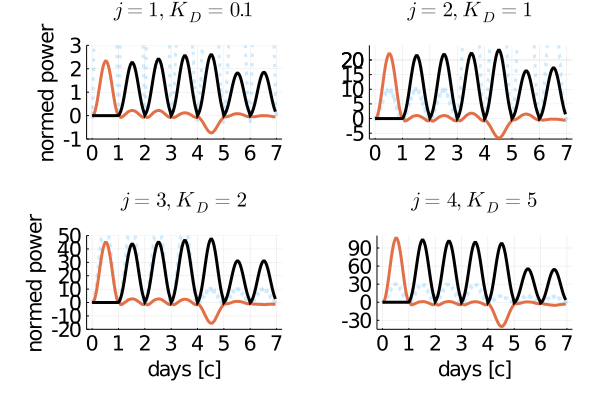
\includegraphics[scale=0.55]{pictures/plots/manual_calc_variation_kappa/kappa_1/K_variance/KDa/DC_prosumer_demand_seconds_nodes_hetero.png}



	\caption{Top: sum for all nodes $j = 1,2,3,4$, $\kappa = \SI{1}{\hour ^{-1}}$ and $\boldsymbol{K_{D,a}} = (0.1,1,2,5)^T\si{\ohm ^{-1}}$; transparent blue: $\sum_{j} P_j^d$, dashed red: $\sum_{j} y_j^{c,h}$, solid black: $\sum_{j}u_j^{ILC}$; Bottom: seperately for nodes $j = 1,2,3,4$, $\kappa = \SI{1}{\hour ^{-1}}$, $\boldsymbol{K_{D,a}} = (0.1,1,2,5)^T\si{\ohm ^{-1}}$; transparent blue: $P_j^d$, solid red: $y_j^{c,h}$, solid black: $u_j^{ILC}$}
	\label{fig:k1_KDa}
\end{figure}

\subsubsection*{Interpretation}
The higher the droop coefficient is, the smaller is the difference between the two voltages. A higher droop coefficient also means a faster reaction of the currents, resulting increasing currents. The low-level control energy per node increases for increasing $K_{D,j}$ and decreases for decreasing $K_{D,j}$, respectively.
\\The sum of the low-layer control energy at every node of the nonlinear model $y^{c,h,s} = \sum_{j}y^{c,h}_j$ with the parameters of Table \ref{tab:parameters} is for every $K_{D,j}\in \mathbb{R}_{>0}$ equal. Changing the droop coefficient in a heterogenous scenario will only change the distribution of the integrated energies on every node and therefore the value of integrated energies per node.
A higher droop coefficient at a node will increase the lower-layer control energy there and reduce it on the rest of the nodes. Likewise the reduction of the droop coefficient at a node will increase the energy of the other nodes. The sum of powers at every node is distributed on all nodes proportionally, depending on the coefficient. 
For every heterogenous scenario the following relationship arises:
\begin{align}
\sum_{j}^{N} K_{D,j} \cdot y^{c,h}_j = y^{c,h,s},N \in \mathcal{N} \subseteq \mathbb{N},j&={1,2,...,N},K_{D,j} \in \mathbb{R}_{>0} \label{eq:sum_energy_het} \\
0.1 \cdot y^{c,h}_1 + y^{c,h}_2 + 2 \cdot y^{c,h}_3 + 5 \cdot y^{c,h}_4 &= y^{c,h,s}, j=1,2,3,4, N=4, \boldsymbol{K_{D}} = \boldsymbol{K_{D,a}} \nonumber  \\
y^{y,h}_1 + y^{c,h}_2 + 0.1 \cdot y^{c,h}_3 + y^{c,h}_4 &= y^{c,h,s},j=1,2,3,4, N=4, \boldsymbol{K_{D}} = \boldsymbol{K_{D,b}} \nonumber
\end{align}
Fair power sharing is achieved for all prosumers. This is necessary in order to assure the same rights for each user regardless of the position in the microgrid. In other words, when a prosumer of the grid feeds a greater amount of power into the grid, the other prosumer will feed a equivalently smaller amount of power intro the grid, to keep the total energy balance of the microgrid.
\\As also in Case 1 ($K_{D,j} = \SI{1}{\hour^{-1}}$), the peak demand steps after four days and again after 3 days and is different at each node (Figures \ref{fig:k1_KDa} and \ref{fig:k1_KDb},bottom). The local ILC learns to compensate the new local demand after each demand peak step, stepping with the same frequency as the local demand and the low-level control energy decreases also after the day after the ILC has learned the new periodic demand. 
\\The next case varies the learning parameter $\kappa$ for a constant droop coefficient $K_{D,j}= \SI{1}{\ohm^{-1}}$ to analyze the learning behavior of the iterative learning controller.
\begin{figure}[h]
	\centering
	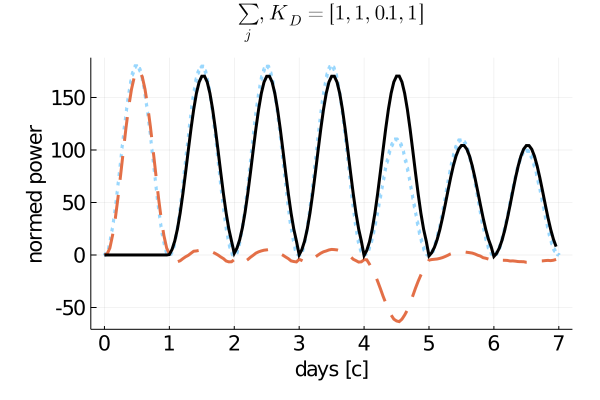
\includegraphics[scale=0.55]{pictures/plots/manual_calc_variation_kappa/kappa_1/K_variance/KDb/DC_prosumer_demand_seconds_sum_hetero.png}
	
	\bigbreak
	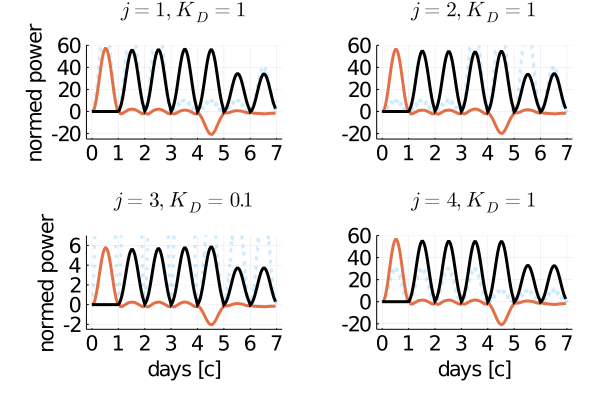
\includegraphics[scale=0.55]{pictures/plots/manual_calc_variation_kappa/kappa_1/K_variance/KDb/DC_prosumer_demand_seconds_nodes_hetero.png}
	
	
	
	\caption{Top: sum for all nodes $j = 1,2,3,4$, $\kappa = \SI{1}{\hour ^{-1}}$ and $\boldsymbol{K_{D,b}} = (1,1,0.1,1)^T\si{\ohm ^{-1}}$; transparent blue: $\sum_{j} P_j^d$, dashed red: $\sum_{j} y_j^{c,h}$, solid black: $\sum_{j}u_j^{ILC}$; Bottom: seperately for nodes $j = 1,2,3,4$, $\kappa = \SI{1}{\hour ^{-1}}$, $\boldsymbol{K_{D,b}} = (1,1,0.1,1)^T\si{\ohm ^{-1}}$; transparent blue: $P_j^d$, solid red: $y_j^{c,h}$, solid black: $u_j^{ILC}$}
	\label{fig:k1_KDb}
\end{figure}
\subsection{Case 3: Variation of  $\boldsymbol{\kappa}$ and $\boldsymbol{K_{D,j}= \SI{1}{\ohm^{-1}}}$}
\label{subsec:case3}
\label{subsec:K_1_kappa_var}
Case 3 serves the purpose of analyzing the learning behavior of the hierarchical control for different learning parameter $\kappa \in ]0,2[ \si{hour^{-1}}$. 
\\Figure \ref{fig:kvar_KD1} presents the sum over all nodes of the demand $\sum_{j}P^d_j$, the low-level control energy $\sum_{j}y^{c,h}_j$ and the input from the ILC $\sum_{j} u^{ILC}_j$ for a learning scenario with artificial step changes of the peak demand for a variety of different learning parameter $\kappa$. 
\subsubsection*{Observations}
\paragraph{$\boldsymbol{\kappa \in ]0,1[\si{\hour^{-1}}}$:}
For $\kappa \in ]0,1[\si{\hour^{-1}}$ the ILC power regulates slowly during the second days and learns the first peak of demand. During the fifth day, for $\kappa = \SI{0.25}{\hour^{-1}}$ the ILC has reached almost $70\%$ of the demand and in the next days it regulates to the next amplitude. For $\kappa = \SI{0.5}{\hour^{-1}}$ and $\kappa = \SI{0.75}{\hour^{-1}}$ the learning improves, while the ILC power approaches during the fifth day the peak demand. However, the response for $\kappa \in ]0,1[\si{\hour^{-1}}$ is slower than for $\kappa = \SI{1}{\hour^{-1}}$, where the ILC has reached the amount of the demand power during the second day. 
\\In addition the low-level control energy decreases for $\kappa \in ]0,1[\si{\hour^{-1}}$, with a bigger $\kappa$ having a faster decrease as result. E.g. the sum of low-level control energy over all nodes decreases faster for $\kappa = \SI{0.75}{\hour^{-1}}$ than for $\kappa = \SI{0.5}{\hour^{-1}}$. The negative peak of the energy that is observed for $\kappa = \SI{1}{\hour^{-1}}$ in Figure \ref{fig:k1_K1} grows with an increasing $\kappa$.
\paragraph{$\boldsymbol{\kappa \in ]1,2[\si{\hour^{-1}}}$:}
For $\kappa$ in $]1,2[\si{\hour^{-1}}$  the ILC shows a quick regulation during the second day and learns the first peak of demand. The more $\kappa$ increases the bigger the amount of the power in the second day gets and the more the learning behavior of the ILC downgrades, as it shows a variety of different amplitudes. E.g. in Figure \ref{fig:kvar_KD1} for $\kappa = \SI{1.5}{\hour^{-1}}$  the demand amplitude is $180$ during the four first days and the ILC shows an amplitude of $250$ in the second and an amplitude of approx. $130$ in the third day  For $\kappa = \SI{1}{\hour^{-1}}$  the ILC learn the demand by adapting the amplitudes of $180$ immediately after the first day. 
\\The lower-layer control energy over all nodes decreases in $\mathbb{R}_{>0}$ and increases in $\mathbb{R}_{<0}$ after the first day for all $\kappa = ]1,2[\si{\hour^{-1}}$ , while the negative peak during the fifth day ($\kappa = \SI{1}{\hour^{-1}}$ ) decreases.

\subsubsection*{Interpretation}
If one compares the single representations from Figure \ref{fig:kvar_KD1} with each other, as well as with the representation in Figure \ref{fig:k1_K1}, one quickly notices that in the interval $\kappa \in ]0,1[\si{\hour^{-1}}$ the learning behavior of the iterative learning controller improves for increasing $\kappa$ and deteriorates for increasing $\kappa$ in $]1,2[\si{\hour^{-1}}$. For $\kappa = \SI{1}{\hour^{-1}}$ the learning scenario is the most efficient. The controller reacts sensitive to the change of the demand amplitudes, so that the integrated energy increases again, until the controller has learned the demand. In the next Section it will be studied how the error convergence in the iteration domain depends on the choice of the scalar learning parameter.

\subsection{Error dynamics for different learning gains}
\label{subsec:error_dyn}
We study how the error convergence in the iteration domain depends on the choice of the scalar learning parameter $\kappa$. Again, the nonlinear model with the two-layer control is used with modified demand pattern \cite{paperilc}. The periodic peak demand is between $0.6$ and $\SI{0.9}{\watt / \watt}$ at the different nodes and the fluctuating component varies randomly from day to day within $[-0.7,0.7]$$\si{\watt / \watt}$. The smaller amplitudes of the demand in this case ensure that the increased low-level energy on day 5 from the upper sections  are again minimised. 
\\Different values of $\kappa = [0,2]\si{\hour^{-1}}$  are considered. For each value, the error norm, i.e. a measure of the overall low-level control energy is calculated for each of the 20 first days \cite{paperilc}. Figure \ref{fig:error_norm} shows the results of the study. For $\kappa \in [0,1]$ the error norm converges faster for increasing $\kappa$. The error norm is constant for $\SI{0}{\hour^{-1}}$ (no learning) over the cycles. For $\kappa \in [1,2]$ the error norm converges slower for increasing $\kappa$, i.e the error norm is not converging for $\kappa = \SI{2}{\hour^{-1}}$. The convergence of the error norm is therefore fastest for $\kappa = \SI{1}{\hour^{-1}}$. This observation confirms the statement from Case 3, that for $\kappa = \SI{1}{\hour^{-1}}$ the learning scenario is the optimal. 
\begin{figure}[!tbp]
	\centering
	\begin{minipage}[b]{0.475\textwidth}
		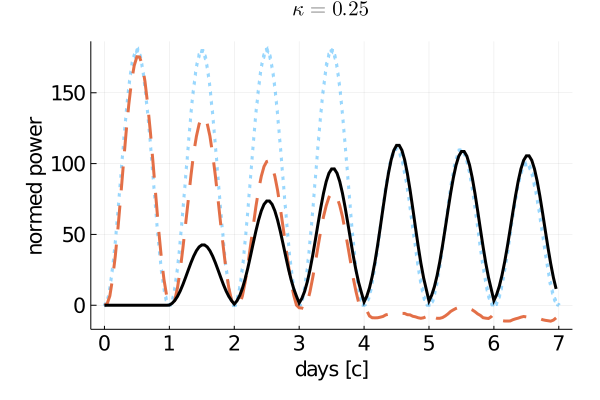
\includegraphics[width=\textwidth]{pictures/plots/manual_calc_variation_kappa/kappa_025_energies_sum.png}
		
	\end{minipage}
	\hfill
	\begin{minipage}[b]{0.475\textwidth}
		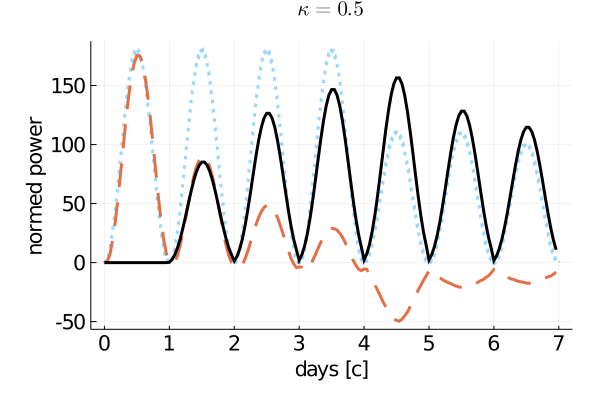
\includegraphics[width=\textwidth]{pictures/plots/manual_calc_variation_kappa/kappa_05_energies_sum.png}
		
	\end{minipage}
\end{figure}
\begin{figure}[!tbp]
	\centering
	\begin{minipage}[b]{0.475\textwidth}
		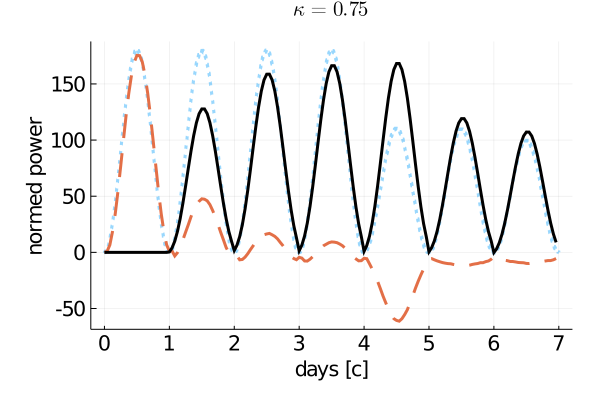
\includegraphics[width=\textwidth]{pictures/plots/manual_calc_variation_kappa/kappa_075_energies_sum.png}
		
	\end{minipage}
	\hfill
	\begin{minipage}[b]{0.475\textwidth}
		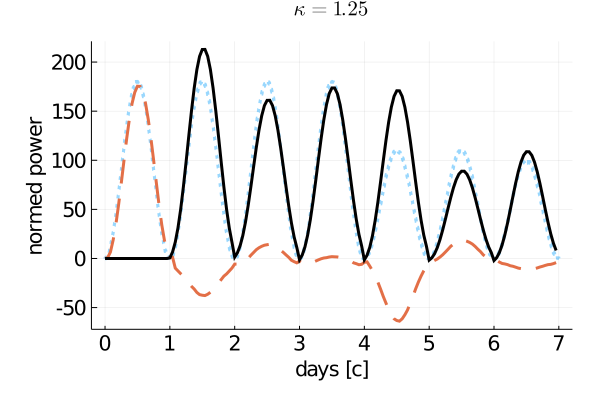
\includegraphics[width=\textwidth]{pictures/plots/manual_calc_variation_kappa/kappa_125_energies_sum.png}
		
	\end{minipage}
\end{figure}
\begin{figure}[!tbp]
	\centering
	\begin{minipage}[b]{0.475\textwidth}
		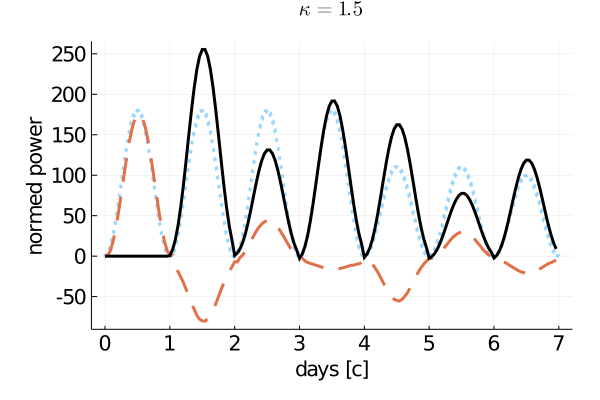
\includegraphics[width=\textwidth]{pictures/plots/manual_calc_variation_kappa/kappa_15_energies_sum.png}
		
	\end{minipage}
	\hfill
	\begin{minipage}[b]{0.475\textwidth}
		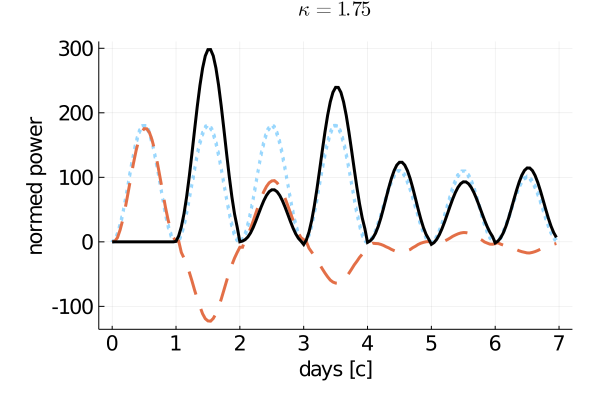
\includegraphics[width=\textwidth]{pictures/plots/manual_calc_variation_kappa/kappa_175_energies_sum.png}
		
	\end{minipage}
	\caption{sum for all nodes $j = 1,2,3,4$ with $K_{D,j} = 1\si{\ohm ^{-1}}$; Top left: $\kappa = \SI{0.25}{\hour ^{-1}}$; Top right: $\kappa = \SI{0.5}{\hour ^{-1}}$; Center left: $\kappa = \SI{0.75}{\hour ^{-1}}$; Center right: $\kappa = \SI{1.25}{\hour ^{-1}}$; Bottom left: $\kappa = \SI{1.5}{\hour ^{-1}}$; Bottom right: $\kappa = \SI{1.75}{\hour ^{-1}}$; transparent blue: $\sum_{j} P_j^d$, dashed red: $\sum_{j} y_j^{c,h}$, solid black: $\sum_{j}u_j^{ILC}$;}
	\label{fig:kvar_KD1}
\end{figure}
\begin{figure}[h]
	\centering
	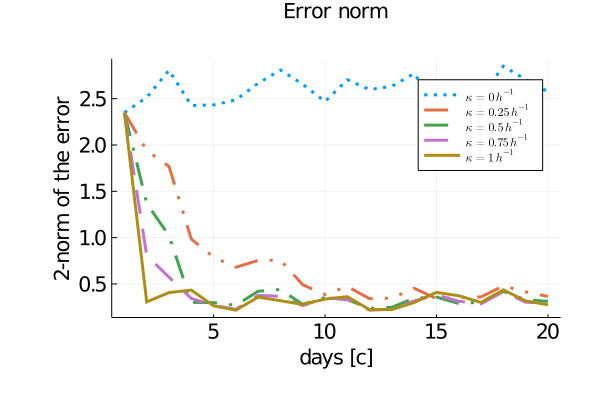
\includegraphics[scale=0.6]{pictures/plots/manual_calc_variation_kappa/variation_kappa_leq_1_hetero.png}
	\bigbreak
	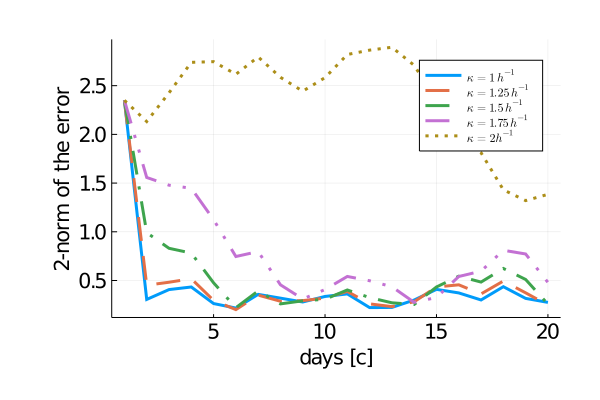
\includegraphics[scale=0.6]{pictures/plots/manual_calc_variation_kappa/variation_kappa_geq_1_hetero.png}
	\caption{Error norm ($||\boldsymbol{e}^c||_2$) over the days for different learning gains with the nonlinear simulation}
	\label{fig:error_norm}
\end{figure} 

\section{Discussion}
Taking all results from Sections \ref{sec:valid_no_ILC} and \ref{sec:valid_ILC} for the prosumer-based direct current microgrid with iterative learning control, it can be said that:
\begin{enumerate}
	\item The suggested prosumer-based direct current microgrid framework (Eq. \ref{eq:system}) with lower-layer control (Eq. \ref{eq:ll_energy}) achieves voltage droop and power sharing with the corresponding droop coefficient $\boldsymbol{K_{D}}$. Depending on the individual purposes, e.g. if a specific prosumer should produce/consume a bigger amount of power, the coefficient, as well as the compound plant parameters can be varied. For an equal distribution of power inbetween the nodes, choosing for the droop coefficient $K_{D,j} = \SI{1}{\ohm^{-1}}$ will complete this purpose.
	\item The suggested iterative learning controller (Eq. \ref{eq:control_ilc}) not only learned the local demand and contributed with the low-level controller by ensuring the power sharing. Instead, it saved the low-level control energy, showing some sensitivity, whenever the peak demand changed.
	\item The low-level control energy was decreased for almost every learning parameter $\kappa$. By calculating the error convergence for the low-level control energy, it was showed that the optimal learning behavior is achieved at $\kappa = \SI{1}{\hour^{-1}}$. 
\end{enumerate}
